\documentclass[a4paper, 11pt]{article}
\usepackage{fullpage} % changes the margin
\usepackage{graphicx}
\usepackage{amsmath}
\usepackage{amssymb}
\usepackage{subfig}

\usepackage{graphicx}
\graphicspath{ {../} }

\usepackage{listings}
\usepackage{color}


\definecolor{dkgreen}{rgb}{0,0.6,0}
\definecolor{gray}{rgb}{0.5,0.5,0.5}
\definecolor{mauve}{rgb}{0.58,0,0.82}

\lstset{frame=tb,
  language=Python,
  aboveskip=3mm,
  belowskip=3mm,
  showstringspaces=false,
  columns=flexible,
  basicstyle={\small\ttfamily},
  numbers=none,
  numberstyle=\tiny\color{gray},
  keywordstyle=\color{blue},
  commentstyle=\color{dkgreen},
  stringstyle=\color{mauve},
  breaklines=true,
  breakatwhitespace=true,
  tabsize=4
}

\begin{document}
	%Header-Make sure you update this information!!!!
	\noindent
	{\Huge\textbf{Graphics Assignment - 1}} \\ \\
	\Large Piyush Chauhan (1701CS33)  \hfill 15th Jan 2020\\ 

	
	\section*{Introduction}
	This task of this assignment is to install OpenGL libraries and test it with Python by drawing simple 2D shapes like rectangle and triangle.


	\section*{Procedure}
	\subsection*{Installation}
	For Ubuntu, the installation involves executing the following commands in the bash:
	\begin{lstlisting}
sudo apt-get update
sudo apt-get install libglu1-mesa-dev freeglut3-dev mesa-common-dev
	\end{lstlisting}

	\subsection*{Policy}
	\begin{enumerate}
		\item Import necessary libraries
		\item Initialize GLUT
		\item Initialize window
		\item Write draw functions for different shapes
		\item Display the shapes 
		\item Loop the drawing for continuous display on the screen. 
	\end{enumerate}

	\section*{Code}
	Python code to create a solid rectangle and a triangle


\begin{lstlisting}
from OpenGL.GL import *
from OpenGL.GLUT import *
from OpenGL.GLU import *

window = 0                                             # glut window number
width, height = 500, 400                               # window size

def draw():                                            # ondraw is called all the time
    glClear(GL_COLOR_BUFFER_BIT | GL_DEPTH_BUFFER_BIT)  # clear the screen
    glLoadIdentity()                                   # reset position
    refresh2d(width, height)                           # set mode to 2d

    glColor3f(0.0, 0.0, 1.0)                           # set color to blue
    # rect at (10, 10) with width 200, height 100
    draw_rect(10, 10, 200, 100)
    draw_triangle([150, 200, 250], [150, 200, 150])
    # important for double buffering
    glutSwapBuffers()

def refresh2d(width, height):
    glViewport(0, 0, width, height)
    glMatrixMode(GL_PROJECTION)
    glLoadIdentity()
    glOrtho(0.0, width, 0.0, height, 0.0, 1.0)
    glMatrixMode(GL_MODELVIEW)
    glLoadIdentity()

def draw_rect(x, y, width, height):
    # start drawing a rectangle
    glBegin(GL_QUADS)
    glVertex2f(x, y)                                   # bottom left point
    glVertex2f(x + width, y)                           # bottom right point
    glVertex2f(x + width, y + height)                  # top right point
    glVertex2f(x, y + height)                          # top left point
    glEnd()                                            # done drawing a rectangle

def draw_triangle(x, y):
    glBegin(GL_LINE_LOOP)
    for i in range(3):
        glVertex2f(x[i], y[i])
    glEnd()

# initialization
glutInit()                                             # initialize glut
glutInitDisplayMode(GLUT_RGBA | GLUT_DOUBLE | GLUT_ALPHA | GLUT_DEPTH)
glutInitWindowSize(width, height)                      # set window size
# set window position
glutInitWindowPosition(250, 200)
# create window with title
window = glutCreateWindow("Graphics Assignment 1")
# set draw function callback
glutDisplayFunc(draw)
glutIdleFunc(draw)                                     # draw all the time
glutMainLoop()                                         # start everything
\end{lstlisting}


	\section*{Output}
	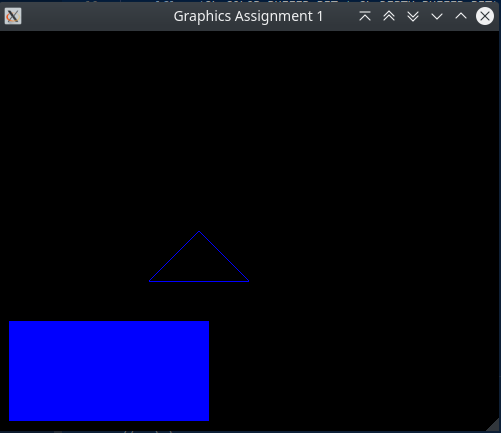
\includegraphics[scale=0.5]{graphicsAssign1}
	
	
\end{document}